\documentclass[a4paper]{article}
\usepackage[a4paper,margin=25mm]{geometry}
\usepackage{graphicx,subcaption}
\usepackage{amsmath,amsfonts}
\usepackage{qtree}
\usepackage{tikz}
\usetikzlibrary{arrows}
\usetikzlibrary{arrows.meta}
\usepackage{varwidth}

\begin{document}
\begin{figure}[hbt]
\centering
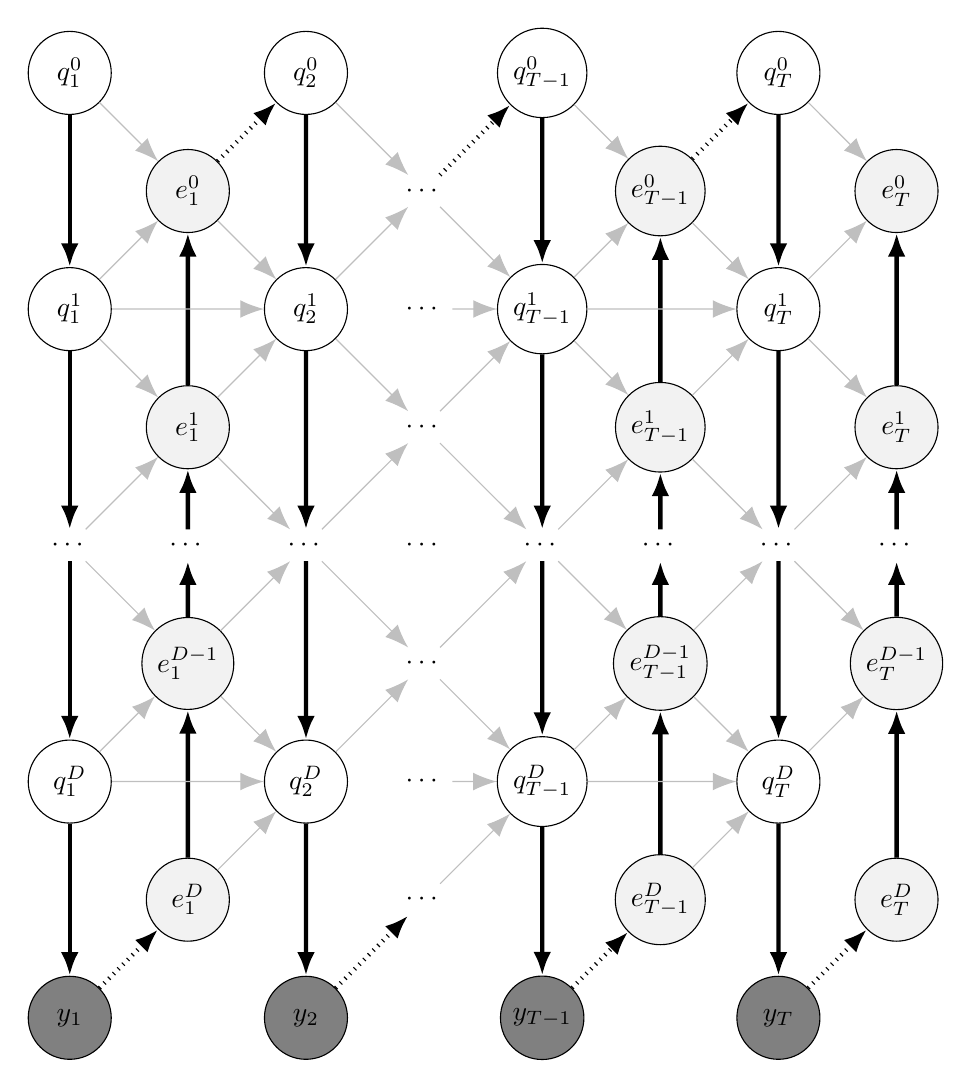
\begin{tikzpicture}[scale=1.5,
cnode/.style={draw,circle,minimum size=3em,inner sep=3pt},
onode/.style={fill=black!50, draw,circle,minimum size=3em,inner sep=3pt},
enode/.style={fill=black!5, draw,circle,minimum size=3em,inner sep=3pt}]
    % down stage 1 states:
    \node[cnode] (q01) at (0,8) {$q^0_1$};
    \node[cnode] (q11) at (0,6) {$q^1_1$};
    \node (qd1) at (0,4) {$\cdots$};
    \node[cnode] (qD1) at (0,2) {$q^D_1$};
    \node[onode] (y1) at (0,0) {$y_1$};
    \draw[-{Latex[length=3mm]}, ultra thick] (q01) edge (q11);
    \draw[-{Latex[length=3mm]}, ultra thick] (q11) edge (qd1);
    \draw[-{Latex[length=3mm]}, ultra thick] (qd1) edge (qD1);
    \draw[-{Latex[length=3mm]}, ultra thick] (qD1) edge (y1);
    % across to stage 1 indicators and up:
    \node[enode] (e01) at (1,7) {$e^0_1$};
    \node[enode] (e11) at (1,5) {$e^1_1$};
    \node (ed1) at (1,4) {$\cdots$};
    \node[enode] (eDm11) at (1,3) {$e^{D-1}_1$};
    \node[enode] (eD1) at (1,1) {$e^{D}_1$};
    \draw[-{Latex[length=3mm]}, lightgray] (q01) edge (e01);
    \draw[-{Latex[length=3mm]}, lightgray] (q11) edge (e01);
    \draw[-{Latex[length=3mm]}, ultra thick] (e11) edge (e01);
    \draw[-{Latex[length=3mm]}, lightgray] (q11) edge (e11);
    \draw[-{Latex[length=3mm]}, lightgray] (qd1) edge (e11);
    \draw[-{Latex[length=3mm]}, ultra thick] (ed1) edge (e11);
    \draw[-{Latex[length=3mm]}, ultra thick] (eDm11) edge (ed1);
    \draw[-{Latex[length=3mm]}, lightgray] (qd1) edge (eDm11);
    \draw[-{Latex[length=3mm]}, lightgray] (qD1) edge (eDm11);
    \draw[-{Latex[length=3mm]}, ultra thick] (eD1) edge (eDm11);

    % down stage 2 states:
    \node[cnode] (q02) at (2,8) {$q^0_2$};
    \node[cnode] (q12) at (2,6) {$q^1_2$};
    \node (qd2) at (2,4) {$\cdots$};
    \node[cnode] (qD2) at (2,2) {$q^D_2$};
    \node[onode] (y2) at (2,0) {$y_2$};
    \draw[-{Latex[length=3mm]}, ultra thick] (q02) edge (q12);
    \draw[-{Latex[length=3mm]}, lightgray] (q11) edge (q12);
    \draw[-{Latex[length=3mm]}, lightgray] (e01) edge (q12);
    \draw[-{Latex[length=3mm]}, lightgray] (e11) edge (q12);
    \draw[-{Latex[length=3mm]}, ultra thick] (q12) edge (qd2);
    \draw[-{Latex[length=3mm]}, lightgray] (e11) edge (qd2);
    \draw[-{Latex[length=3mm]}, lightgray] (eDm11) edge (qd2);
    \draw[-{Latex[length=3mm]}, ultra thick] (qd2) edge (qD2);
    \draw[-{Latex[length=3mm]}, lightgray] (qD1) edge (qD2);
    \draw[-{Latex[length=3mm]}, lightgray] (eDm11) edge (qD2);
    \draw[-{Latex[length=3mm]}, lightgray] (eD1) edge (qD2);
    \draw[-{Latex[length=3mm]}, ultra thick] (qD2) edge (y2);

    % stage t
    \node (e0t) at (3,7) {$\cdots$};
    \node (q1t) at (3,6) {$\cdots$};
    \node (e1t) at (3,5) {$\cdots$};
    \node (qDm1t) at (3,4) {$\cdots$};
    \node (eDm1t) at (3,3) {$\cdots$};
    \node (qDt) at (3,2) {$\cdots$};
    \node (eDt) at (3,1) {$\cdots$};
    \draw[-{Latex[length=3mm]}, lightgray] (q02) edge (e0t);
    \draw[-{Latex[length=3mm]}, lightgray] (q12) edge (e0t);
    \draw[-{Latex[length=3mm]}, lightgray] (q12) edge (e1t);
    \draw[-{Latex[length=3mm]}, lightgray] (qd2) edge (e1t);
    \draw[-{Latex[length=3mm]}, lightgray] (qd2) edge (eDm1t);
    \draw[-{Latex[length=3mm]}, lightgray] (qD2) edge (eDm1t);

    % down stage T-1 states:
    \node[cnode] (q0Tm1) at (4,8) {$q^0_{T-1}$};
    \node[cnode] (q1Tm1) at (4,6) {$q^1_{T-1}$};
    \node (qdTm1) at (4,4) {$\cdots$};
    \node[cnode] (qDTm1) at (4,2) {$q^D_{T-1}$};
    \node[onode] (yTm1) at (4,0) {$y_{T-1}$};
    \draw[-{Latex[length=3mm]}, ultra thick] (q0Tm1) edge (q1Tm1);
    \draw[-{Latex[length=3mm]}, lightgray] (q1t) edge (q1Tm1);
    \draw[-{Latex[length=3mm]}, lightgray] (e0t) edge (q1Tm1);
    \draw[-{Latex[length=3mm]}, lightgray] (e1t) edge (q1Tm1);
    \draw[-{Latex[length=3mm]}, ultra thick] (q1Tm1) edge (qdTm1);
    \draw[-{Latex[length=3mm]}, lightgray] (e1t) edge (qdTm1);
    \draw[-{Latex[length=3mm]}, lightgray] (eDm1t) edge (qdTm1);
    \draw[-{Latex[length=3mm]}, ultra thick] (qdTm1) edge (qDTm1);
    \draw[-{Latex[length=3mm]}, lightgray] (qDt) edge (qDTm1);
    \draw[-{Latex[length=3mm]}, lightgray] (eDm1t) edge (qDTm1);
    \draw[-{Latex[length=3mm]}, lightgray] (eDt) edge (qDTm1);
    \draw[-{Latex[length=3mm]}, ultra thick] (qDTm1) edge (yTm1);
    % across to stage T-1 indicators and up:
    \node[enode] (e0Tm1) at (5,7) {$e^0_{T-1}$};
    \node[enode] (e1Tm1) at (5,5) {$e^1_{T-1}$};
    \node (edTm1) at (5,4) {$\cdots$};
    \node[enode] (eDm1Tm1) at (5,3) {$e^{D-1}_{T-1}$};
    \node[enode] (eDTm1) at (5,1) {$e^{D}_{T-1}$};
    \draw[-{Latex[length=3mm]}, lightgray] (q0Tm1) edge (e0Tm1);
    \draw[-{Latex[length=3mm]}, lightgray] (q1Tm1) edge (e0Tm1);
    \draw[-{Latex[length=3mm]}, ultra thick] (e1Tm1) edge (e0Tm1);
    \draw[-{Latex[length=3mm]}, lightgray] (q1Tm1) edge (e1Tm1);
    \draw[-{Latex[length=3mm]}, lightgray] (qdTm1) edge (e1Tm1);
    \draw[-{Latex[length=3mm]}, ultra thick] (edTm1) edge (e1Tm1);
    \draw[-{Latex[length=3mm]}, ultra thick] (eDm1Tm1) edge (edTm1);
    \draw[-{Latex[length=3mm]}, lightgray] (qdTm1) edge (eDm1Tm1);
    \draw[-{Latex[length=3mm]}, lightgray] (qDTm1) edge (eDm1Tm1);
    \draw[-{Latex[length=3mm]}, ultra thick] (eDTm1) edge (eDm1Tm1);

    % down stage T states:
    \node[cnode] (q0T) at (6,8) {$q^0_{T}$};
    \node[cnode] (q1T) at (6,6) {$q^1_{T}$};
    \node (qdT) at (6,4) {$\cdots$};
    \node[cnode] (qDT) at (6,2) {$q^D_{T}$};
    \node[onode] (yT) at (6,0) {$y_{T}$};
    \draw[-{Latex[length=3mm]}, ultra thick] (q0T) edge (q1T);
    \draw[-{Latex[length=3mm]}, lightgray] (q1Tm1) edge (q1T);
    \draw[-{Latex[length=3mm]}, lightgray] (e0Tm1) edge (q1T);
    \draw[-{Latex[length=3mm]}, lightgray] (e1Tm1) edge (q1T);
    \draw[-{Latex[length=3mm]}, ultra thick] (q1T) edge (qdT);
    \draw[-{Latex[length=3mm]}, lightgray] (e1Tm1) edge (qdT);
    \draw[-{Latex[length=3mm]}, lightgray] (eDm1Tm1) edge (qdT);
    \draw[-{Latex[length=3mm]}, ultra thick] (qdT) edge (qDT);
    \draw[-{Latex[length=3mm]}, lightgray] (qDTm1) edge (qDT);
    \draw[-{Latex[length=3mm]}, lightgray] (eDm1Tm1) edge (qDT);
    \draw[-{Latex[length=3mm]}, lightgray] (eDTm1) edge (qDT);
    \draw[-{Latex[length=3mm]}, ultra thick] (qDT) edge (yT);
    % across to stage T indicators and up:
    \node[enode] (e0T) at (7,7) {$e^0_{T}$};
    \node[enode] (e1T) at (7,5) {$e^1_{T}$};
    \node (edT) at (7,4) {$\cdots$};
    \node[enode] (eDm1T) at (7,3) {$e^{D-1}_{T}$};
    \node[enode] (eDT) at (7,1) {$e^{D}_{T}$};
    \draw[-{Latex[length=3mm]}, lightgray] (q0T) edge (e0T);
    \draw[-{Latex[length=3mm]}, lightgray] (q1T) edge (e0T);
    \draw[-{Latex[length=3mm]}, ultra thick] (e1T) edge (e0T);
    \draw[-{Latex[length=3mm]}, lightgray] (q1T) edge (e1T);
    \draw[-{Latex[length=3mm]}, lightgray] (qdT) edge (e1T);
    \draw[-{Latex[length=3mm]}, ultra thick] (edT) edge (e1T);
    \draw[-{Latex[length=3mm]}, ultra thick] (eDm1T) edge (edT);
    \draw[-{Latex[length=3mm]}, lightgray] (qdT) edge (eDm1T);
    \draw[-{Latex[length=3mm]}, lightgray] (qDT) edge (eDm1T);
    \draw[-{Latex[length=3mm]}, ultra thick] (eDT) edge (eDm1T);

    % special
    \begin{scope}[dotted]
      \draw[-{Latex[length=3mm]}, ultra thick] (e01) to (q02);
      \draw[-{Latex[length=3mm]}, ultra thick] (y1) to (eD1);
      \draw[-{Latex[length=3mm]}, ultra thick] (y2) to (eDt);
      \draw[-{Latex[length=3mm]}, ultra thick] (e0t) to (q0Tm1);
      \draw[-{Latex[length=3mm]}, ultra thick] (yTm1) to (eDTm1);
      \draw[-{Latex[length=3mm]}, ultra thick] (e0Tm1) to (q0T);
      \draw[-{Latex[length=3mm]}, ultra thick] (yT) to (eDT);
    \end{scope}
\end{tikzpicture}
\end{figure}

\end{document}
